\documentclass[notes]{beamer}          % print frame + notes
%\documentclass[notes=only]{beamer}     % only notes
%\documentclass{beamer}                 % only frames

\usecolortheme{beaver}

% Some commonly used packages
% (copied mainly from the Utrecht University theme: https://www.overleaf.com/project/5c900fa3bd9930036341116a)
\usepackage{ragged2e}  % `\justifying` text
\usepackage{booktabs}  % Tables
\usepackage{tabularx}
\usepackage{tikz}      % Diagrams
\usetikzlibrary{calc, shapes, backgrounds}
\usepackage{amsmath, amssymb, amsfonts, amsthm}
\usepackage{url}       % `\url`s
\usepackage{listings}  % Code listings
\usepackage{comment}
\usepackage{mathtools}
\usepackage{graphicx}
\usepackage{subfig}
\usepackage{bm}

% Mainly math commands
\newcommand{\vect}[1]{\bm{#1}}
\usepackage{amsfonts}% to get the \mathbb alphabet
\newcommand{\field}[1]{\mathbb{#1}}
\newcommand{\C}{\field{C}}
\newcommand{\R}{\field{R}}
\newcommand{\norm}[1]{\left\lVert#1\right\rVert}
\newcommand{\argmin}{\operatornamewithlimits{argmin}}
\providecommand{\abs}[1]{\lvert#1\rvert}
\providecommand{\norm}[1]{\lVert#1\rVert}

% A variable used to exclude slides from the lecture version
\newif\iffull
%\fullfalse
\fulltrue

% Bibliography
\usepackage[uniquename=init,giveninits=true,maxcitenames=1,style=authortitle-comp]{biblatex}
\bibliography{lectures/references}

%Information to be included in the title page:
\title{Course introduction 2020}
\author{Mitko Veta, Federica Eduati}
\institute{Eindhoven University of Technology

Department of Biomedical Engineering}
\date{2020}
 
 
 
\begin{document}
 
\frame{\titlepage}

\begin{frame}
\frametitle{Why machine learning?}
\begin{center}

\includegraphics[height=7cm]{../figures/intro/machine_learning.png}
\end{center}
{\tiny Figure source: xkcd.com}
\end{frame}

\begin{frame}
\frametitle{Historical perspective}
\begin{center}
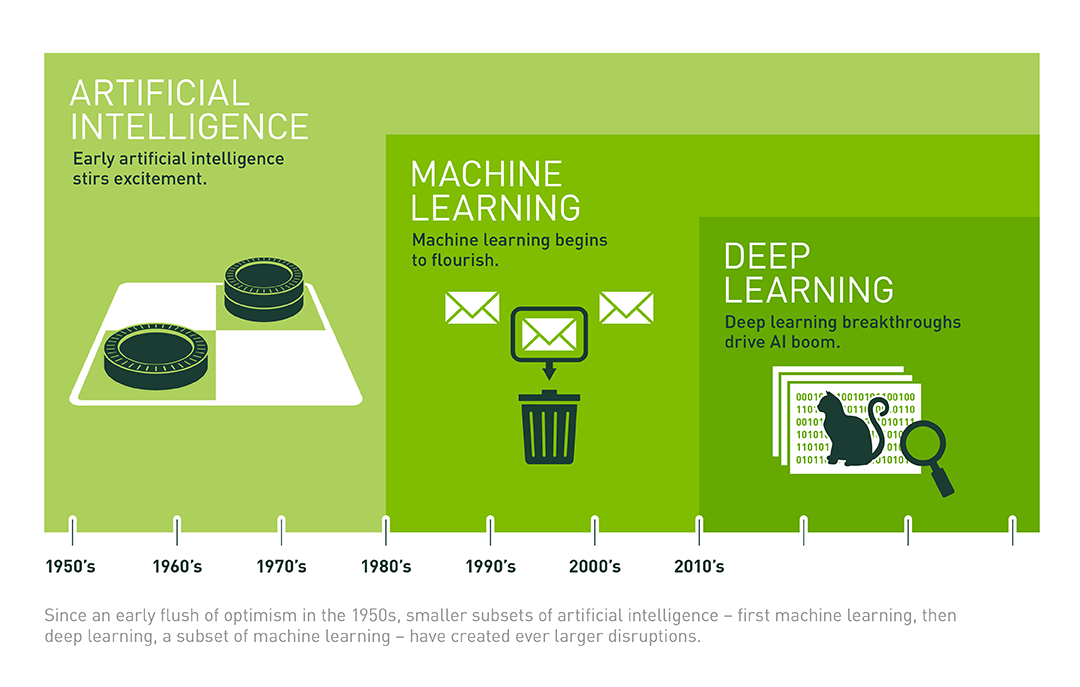
\includegraphics[height=7cm]{../figures/intro/deep_learning.png}
\end{center}
{\tiny Figure source: nvidia.com}
\end{frame}

\begin{frame}{Topics covered in the course}
\begin{itemize}
    \item Week 1: Machine learning fundamentals I (Mitko Veta)
    \item Week 2: Machine learning fundamentals II (Mitko Veta)
    \item Week 3: Linear models (Federica Eduati)
    \item Week 4: Deep learning I (Mitko Veta)
    \item Week 5: Deep learning II (Jelmer Wolterink, U Twente)
    \item Week 6: SVM, random forests (Federica Eduati)
    \item Week 7: Unsupervised machine learning (Federica Eduati) 
\end{itemize}
$\,$\\
Weeks 1-6 lecture and practical. Week 7 only lecture.
\end{frame}

\begin{frame}{The course in a nutshell}
\begin{itemize}
    \item{Assessment}
        \begin{itemize}
            \item 65\% written exam
            \item 25\% practicals
            \item 10\% reading assignment
            \item 0\% \textbf{mandatory} Python self-assessment quiz in the first week
        \end{itemize}
    \item GitHub repository used for material dissemination
    \item Canvas used for communication and submissions/grading
    \item Lectures, time: Mondays 13.30 - 15.30, location: Atlas - 1.210 and on-line
    \item Guided self-study, time: Mondays 15.30 - 17.30, location: on-line via Microsoft Teams
    
\end{itemize}
\end{frame}

\begin{frame}{Study materials}
\begin{itemize}
\item Main: lecture slides and practicals
\item Books
\begin{itemize}
    \item \textbf{Deep Learning}, Ian Goodfellow and Yoshua Bengio and Aaron Courville
    \item \textbf{The elements of Statistical Learning}, Trevor Hastie, Robert Tibshirani, Jerome Friedman
\end{itemize}
\item Specific chapters and additional material (such as papers) are referenced in the lecture slides
\end{itemize}
\end{frame}

\begin{frame}{Practicals}
\begin{itemize}
    \item Distributed as Python notebooks
    \item Deliverables
    \begin{itemize}
        \item Python functions and/or classes (.py files) that implement basic functionalities (e.g. a $k$-NN classifier)
        \item A \textbf{single} Python notebook that contains the experiments, visualization and answer to the questions and math problems.
    \end{itemize}
    \item The assessment rubric for the practicals can be found in the handouts for week 1
    \item Instructions to setup the environment are in GitHub
    \item Each group has a teaching assistant that can be contacted via Teams during the practical sessions
    	\item You are encouraged to use Canvas Discussion to ask general questions
\end{itemize}    
\end{frame}

\begin{frame}{Reading assignment}
\begin{itemize}
    \item Select a paper per group with following criteria
    \begin{itemize}
        \item Describes an application of Machine Learning to a Medical Imaging or Computational Biology problem
		\item Recently published (after 2015)
		\item Published in a high-quality journal (reference list in GitHub)
		\item	 On a topic that you find interesting and want to learn more about
    \end{itemize}
    \item Use the 'paper selection' assignment to discuss paper selection with us (propose a list)
    \item Write a review (800 words) with:
    \begin{itemize}
    		\item Summary of the application domain of the paper
    		\item Summary of the used (Machine Learning) methodology and evaluation metrics
		\item Discussion of strong and weak points of the methodology and evaluation metrics
		\item Suggestion of alternative methodology, evaluation metrics and ideas for improvement
    \end{itemize}
\end{itemize}    
\end{frame}

\end{document}
